\documentclass[11pt]{article}
\usepackage{mathtools}
\usepackage{mdframed}
\usepackage{fullpage}
\usepackage{tikz}            % if you delete this, you will have trouble with the included picture. You can delete the picture.




\newcommand\name{John Vincent} %%%%%%%%%%%%%%  WRITE YOUR NAME HERE



\newcounter{excounter}
\setcounter{excounter}{1}
\newcommand\question[2]{\vskip 1em  \noindent\textbf{\arabic{excounter}\addtocounter{excounter}{1}:} \emph{#1} \noindent#2}


% You can also erase this if you do not have package hancyhdr
% Fancy footnote.........
\usepackage{fancyhdr}  %% If it does not work with your latex installation, you may just delete this...
\pagestyle{fancy}
\usepackage{lastpage}
\rfoot{\name, page \thepage/\pageref{LastPage}}
\cfoot{}
\rhead{}
\lhead{}
\renewcommand{\headrulewidth}{0pt}
\renewcommand{\footrulewidth}{0pt}



\begin{document}


{\bf COMS 331  \hspace{1cm} HW 0\hfill \name}
\vskip 2em


%\question{}

\begin{mdframed}
  This is an inline equation: $x + y = 3$.\\
  This is a displayed equation: \begin{equation*}x + \frac{y}{z-\sqrt{3}}=2.\end{equation*}
  This is how you can define a piece-wise linear function:
    \[
      f(x) =
      \begin{cases}
        3x + 2 & \text{if $x < 0$}\\
        7x + 2 & \text{if $x \geq 0$ and $x < 10$}\\
        5x + 22 & \text{otherwise.}
      \end{cases}
    \]
  This is a matrix:
    \bgroup
      \def\arraystretch{1.5}%
      \begin{center}
        \begin{tabular}{|c|c|c|c|}
          \hline
          9 & 9 & 9 & 9 \\ \hline
          6 & 6 & 6 &   \\ \hline
          3 &   & 3 & 3 \\
          \hline
        \end{tabular}
      \end{center}
    \egroup
  This is a figure incorporated in a LaTeX file
  \begin{center}
    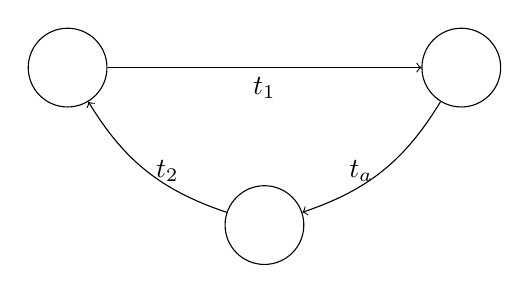
\begin{tikzpicture}
      \node[shape=circle,draw=black,minimum size=1cm] (A) at (0,2) {};
      \node[shape=circle,draw=black,minimum size=1cm] (B) at (5,2) {};
      \node[shape=circle,draw=black,minimum size=1cm] (C) at (2.5,0) {};

      \path [->] (A) edge node[below] {$t_{1}$} (B);
      \path [->] (B) edge[bend left=20] node[left] {$t_{a}$} (C);
      \path [->] (C) edge[bend left=20] node[right] {$t_{2}$} (A);
    \end{tikzpicture}
  \end{center}
\end{mdframed}

\end{document}
